% !TEX program = xelatex
\documentclass[12pt,a4paper]{article}

% Packages
\usepackage[top=1in, bottom=1in, left=1.25in, right=1.25in]{geometry}
\usepackage{times}
\usepackage{graphicx}
\usepackage{setspace}
\usepackage{hyperref}
\usepackage{xcolor}
\usepackage{fancyhdr}
\usepackage{tikz}
\usepackage{pgfplots}
\usepackage{array}
\usepackage{booktabs}
\usepackage{listings}
\usepackage{color}
\usepackage{amsmath}

% TikZ libraries
\usetikzlibrary{shapes.geometric, arrows, positioning, calc, shadows, decorations.pathreplacing}

% Font settings
\usepackage{fontspec}
\setmainfont{Times New Roman}

% Page style
\pagestyle{fancy}
\fancyhf{}
\rfoot{\thepage}
\renewcommand{\headrulewidth}{0pt}

% Line spacing
\onehalfspacing

% Define colors for diagrams
\definecolor{lightblue}{RGB}{173,216,230}
\definecolor{lightgreen}{RGB}{144,238,144}
\definecolor{lightyellow}{RGB}{255,255,224}
\definecolor{lightpink}{RGB}{255,182,193}
\definecolor{lightgray}{RGB}{211,211,211}

% Arrow styles
\tikzstyle{arrow} = [thick,->,>=stealth]
\tikzstyle{line} = [thick,-]

\begin{document}

% ==================== COVER PAGE ====================
\begin{titlepage}
    \centering
    \vspace*{1.5cm}
    
    {\fontsize{16}{20}\selectfont\textbf{PROJECT REPORT}}
    
    \vspace{1cm}
    
    {\fontsize{14}{18}\selectfont\textbf{COSMOS}}
    
    \vspace{0.5cm}
    
    {\fontsize{12}{14}\selectfont\textbf{AI Web Automation Tool - Chrome Extension}}
    
    \vspace{2cm}
    
    {\fontsize{12}{14}\selectfont
    A Free and Privacy-Focused Alternative to Commercial Web Automation Solutions
    }
    
    \vspace{2.5cm}
    
    {\fontsize{12}{14}\selectfont
    \textbf{Project Category:} Browser Extension Development \\
    \vspace{0.3cm}
    \textbf{Technology:} React, TypeScript, Vite \\
    \vspace{0.3cm}
    \textbf{Version:} 0.1.12 \\
    \vspace{0.3cm}
    \textbf{Status:} Production Ready
    }
    
    \vfill
    
    {\fontsize{12}{14}\selectfont
    \textit{Open Source Project} \\
    \vspace{0.2cm}
    GitHub: github.com/cosmos/cosmos \\
    \vspace{0.2cm}
    Chrome Web Store: Available
    }
    
    \vspace{1cm}
    
\end{titlepage}

% ==================== TABLE OF CONTENTS ====================
\newpage
\tableofcontents
\newpage

% ==================== 1. INTRODUCTION ====================
\section*{\textbf{1. INTRODUCTION}}
\addcontentsline{toc}{section}{1. INTRODUCTION}

\setlength{\parindent}{0.5in}

Cosmos is an open-source AI-powered web automation tool designed as a Chrome extension. It enables users to automate complex web workflows using artificial intelligence while maintaining complete privacy and control. Unlike commercial solutions that charge subscription fees, Cosmos is completely free and runs entirely within the user's browser.

\vspace{0.3cm}

The project addresses a critical gap in the market: expensive web automation tools like OpenAI Operator cost \$200+ per month. Cosmos provides equivalent functionality without subscription costs, allowing users to leverage their own API keys and pay only for what they use.

\vspace{0.3cm}

\subsection*{\textbf{1.1 Problem Statement}}

Modern web automation requires intelligent decision-making capabilities that traditional scripting tools cannot provide. Commercial AI automation tools are prohibitively expensive, creating a barrier for individual developers, students, and small businesses. Additionally, existing solutions often compromise user privacy by processing data on external servers.

\vspace{0.3cm}

\subsection*{\textbf{1.2 Proposed Solution}}

Cosmos implements a multi-agent AI system that operates entirely within the browser, ensuring data privacy while providing sophisticated automation capabilities. The system uses specialized agents (Navigator and Thinker) that collaborate to understand context, make decisions, and execute complex workflows.

\vspace{0.3cm}

\subsection*{\textbf{1.3 Key Features}}

\begin{itemize}
    \item \textbf{Multi-Agent AI System:} Specialized agents (Navigator and Thinker) collaborate to solve complex tasks
    \item \textbf{Privacy-First Design:} All processing happens locally in the browser with no data transmission to external servers
    \item \textbf{Flexible LLM Support:} Works with OpenAI, Anthropic, Gemini, Groq, Ollama, and custom providers
    \item \textbf{100\% Free and Open Source:} No hidden costs, subscription fees, or proprietary restrictions
    \item \textbf{Interactive UI:} Real-time chat interface with persistent conversation history
    \item \textbf{Cross-Browser Support:} Full compatibility with Chrome and Microsoft Edge browsers
    \item \textbf{Configurable Cost Controls:} Granular settings to optimize API usage and minimize expenses
    \item \textbf{Advanced DOM Manipulation:} Intelligent interaction with dynamic web content
\end{itemize}

\vspace{0.3cm}

\subsection*{\textbf{1.4 Technical Innovation}}

The project introduces several technical innovations including a browser-native multi-agent architecture, provider-agnostic LLM routing, real-time DOM state management, and a sophisticated action planning system that balances automation accuracy with API cost efficiency.

\vspace{0.3cm}

\subsection*{\textbf{1.5 Target Audience}}

\begin{itemize}
    \item \textbf{Developers:} Automate testing, data extraction, and repetitive development tasks
    \item \textbf{Researchers:} Gather data from multiple sources efficiently
    \item \textbf{Students:} Learn AI integration and browser automation without financial barriers
    \item \textbf{Small Businesses:} Automate workflows without enterprise software costs
    \item \textbf{Privacy-Conscious Users:} Individuals requiring local-first automation solutions
\end{itemize}

\newpage

% ==================== 2. OBJECTIVES ====================
\section*{\textbf{2. OBJECTIVES OF THE STUDY}}
\addcontentsline{toc}{section}{2. OBJECTIVES OF THE STUDY}

The main objectives of the Cosmos project are:

\vspace{0.3cm}

\subsection*{\textbf{2.1 Primary Objectives}}

\begin{enumerate}
    \item \textbf{Democratize Web Automation:} Make advanced AI automation accessible to everyone without expensive subscriptions or enterprise licensing
    
    \item \textbf{Ensure Privacy and Security:} Design a system where user data never leaves their browser, ensuring complete data sovereignty
    
    \item \textbf{Provide Flexibility:} Allow users to choose their preferred AI models and providers based on their specific needs and budget
    
    \item \textbf{Build Multi-Agent Intelligence:} Create specialized agents that can reason, plan, and execute tasks collaboratively with self-correction capabilities
\end{enumerate}

\vspace{0.3cm}

\subsection*{\textbf{2.2 Technical Objectives}}

\begin{enumerate}
    \item \textbf{Create User-Friendly Interface:} Design an intuitive chat-based interface for task automation that requires no programming knowledge
    
    \item \textbf{Maintain Code Quality:} Establish and enforce best practices for open-source development including comprehensive testing and documentation
    
    \item \textbf{Enable Complex Workflows:} Support sophisticated web automation tasks including data extraction, form filling, navigation, and multi-step processes
    
    \item \textbf{Optimize Cost Efficiency:} Provide configuration options to balance performance and API costs through intelligent model selection and action planning
    
    \item \textbf{Ensure Browser Compatibility:} Develop using Manifest V3 standards to ensure long-term compatibility with modern browsers
    
    \item \textbf{Implement Robust Error Handling:} Create self-healing automation that can recover from failures and adapt to changing web interfaces
\end{enumerate}

\vspace{0.3cm}

\subsection*{\textbf{2.3 Community Objectives}}

\begin{enumerate}
    \item \textbf{Foster Open Collaboration:} Build an active community of contributors through Discord, GitHub, and comprehensive documentation
    
    \item \textbf{Educational Impact:} Provide learning resources for AI integration, browser extension development, and modern web technologies
    
    \item \textbf{Continuous Improvement:} Establish feedback loops for rapid iteration and feature development based on user needs
\end{enumerate}

\newpage

% ==================== 3. METHODOLOGY ====================
\section*{\textbf{3. DETAILED METHODOLOGY USED FOR CARRYING OUT THE STUDY}}
\addcontentsline{toc}{section}{3. DETAILED METHODOLOGY USED FOR CARRYING OUT THE STUDY}

\subsection*{\textbf{3.1 System Architecture Overview}}

The Cosmos project employs a layered architecture that separates concerns and enables modular development. The system consists of five primary layers:

\vspace{0.3cm}

\begin{figure}[h]
\centering
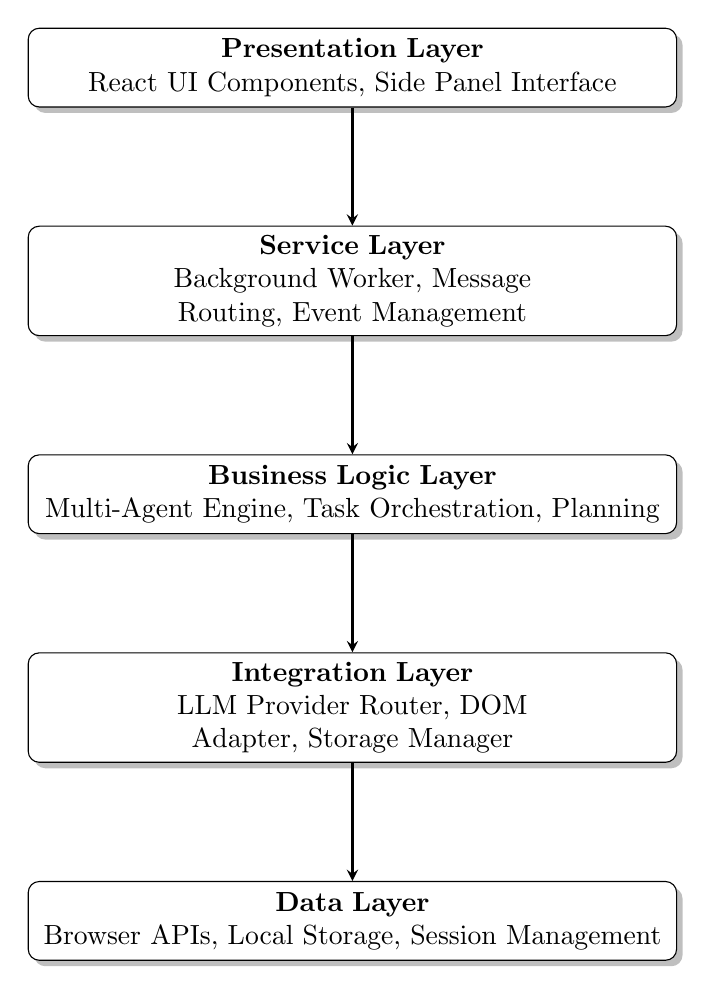
\begin{tikzpicture}[
    node distance=1.5cm,
    box/.style={rectangle, draw, fill=white, text width=8cm, align=center, rounded corners, minimum height=1cm, drop shadow},
    arrow/.style={->, >=stealth, thick}
]
    \node[box] (presentation) {\textbf{Presentation Layer} \\ React UI Components, Side Panel Interface};
    \node[box, below=of presentation, fill=white] (service) {\textbf{Service Layer} \\ Background Worker, Message Routing, Event Management};
    \node[box, below=of service, fill=white] (business) {\textbf{Business Logic Layer} \\ Multi-Agent Engine, Task Orchestration, Planning};
    \node[box, below=of business, fill=white] (integration) {\textbf{Integration Layer} \\ LLM Provider Router, DOM Adapter, Storage Manager};
    \node[box, below=of integration, fill=white] (data) {\textbf{Data Layer} \\ Browser APIs, Local Storage, Session Management};
    
    \draw[arrow] (presentation) -- (service);
    \draw[arrow] (service) -- (business);
    \draw[arrow] (business) -- (integration);
    \draw[arrow] (integration) -- (data);
\end{tikzpicture}
\caption{Layered Architecture of Cosmos System}
\end{figure}
\newpage

\subsection*{\textbf{3.2 Detailed Component Architecture}}

\begin{figure}[h]
\centering
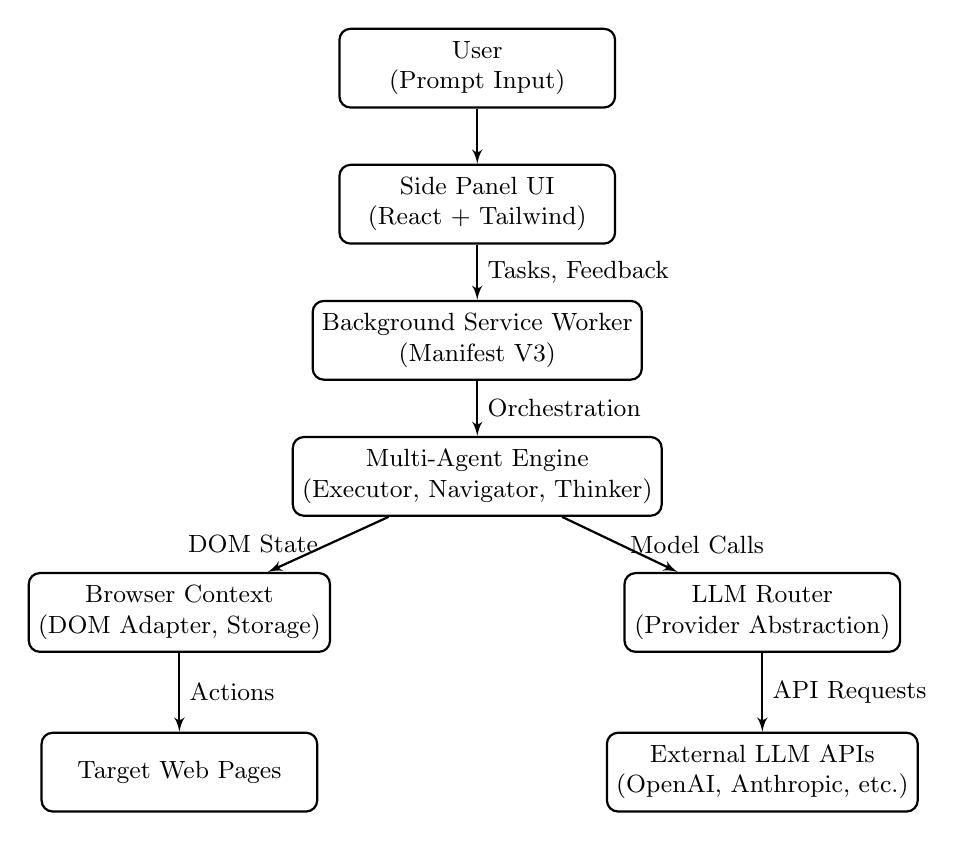
\begin{tikzpicture}[
    node distance=.7cm,
    every node/.style={font=\small, align=center},
    block/.style={rectangle, rounded corners, draw=black, thick, minimum width=3.5cm, minimum height=1cm, fill=white},
    line/.style={draw, -latex', thick}
]
    % Top level
    \node[block, fill=white] (user) {User \\ (Prompt Input)};
    \node[block, fill=white, below=of user] (ui) {Side Panel UI \\ (React + Tailwind)};
    \node[block, fill=white, below=of ui] (serviceworker) {Background Service Worker \\ (Manifest V3)};
    \node[block, fill=white, below=of serviceworker] (agent) {Multi-Agent Engine \\ (Executor, Navigator, Thinker)};
    \node[block, fill=white, below left=.7cm and -0.5cm of agent] (browserctx) {Browser Context \\ (DOM Adapter, Storage)};
    \node[block, fill=white, below right=.7cm and -0.5cm of agent] (llmrouter) {LLM Router \\ (Provider Abstraction)};
    \node[block, fill=white, below=1cm of browserctx] (web) {Target Web Pages};
    \node[block, fill=white, below=1cm of llmrouter] (llms) {External LLM APIs \\ (OpenAI, Anthropic, etc.)};

    % Connections
    \path[line] (user) -- (ui);
    \path[line] (ui) -- node[right]{Tasks, Feedback} (serviceworker);
    \path[line] (serviceworker) -- node[right]{Orchestration} (agent);
    \path[line] (agent) -- node[left]{DOM State} (browserctx);
    \path[line] (agent) -- node[right]{Model Calls} (llmrouter);
    \path[line] (browserctx) -- node[right]{Actions} (web);
    \path[line] (llmrouter) -- node[right]{API Requests} (llms);
\end{tikzpicture}
\caption{Detailed Component Architecture and Data Flow}
\end{figure}

\subsection*{\textbf{3.3 Technology Stack and Justification}}

\begin{table}[h]
\centering
\begin{tabular}{|l|l|p{6cm}|}
\hline
\textbf{Component} & \textbf{Technology} & \textbf{Justification} \\
\hline
Frontend Framework & React 18.3.1 & Component reusability, virtual DOM, hooks for state management \\
\hline
Language & TypeScript 5.5.4 & Type safety, better IDE support, reduced runtime errors \\
\hline
Build Tool & Vite 6.3.6 & Fast HMR, optimized bundling, modern ESM support \\
\hline
Styling & Tailwind CSS 3.4.17 & Utility-first approach, consistent design, small bundle size \\
\hline
Package Manager & pnpm 9.15.1 & Disk space efficiency, faster installation, monorepo support \\
\hline
\end{tabular}
\caption{Technology Stack with Justifications}
\end{table}
\newpage

\subsection*{\textbf{3.4 Multi-Agent System Design}}

The automation engine implements a collaborative multi-agent architecture:

\vspace{0.3cm}

\textbf{Navigator Agent:}
\begin{itemize}
    \item Responsible for direct web page interactions
    \item Executes actions: clicks, form filling, scrolling, data extraction
    \item Maintains browser state and DOM snapshots
    \item Implements retry logic for failed actions
\end{itemize}

\vspace{0.3cm}

\textbf{Thinker Agent:}
\begin{itemize}
    \item Plans task execution strategies
    \item Reasons about complex problems and edge cases
    \item Provides self-correction and error recovery
    \item Determines task completion criteria
\end{itemize}

\vspace{0.3cm}

\begin{figure}[h]
\centering
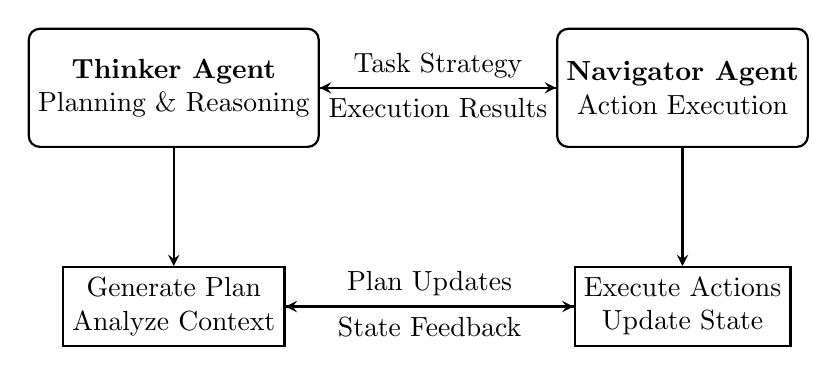
\begin{tikzpicture}[
    node distance=3cm,
    agent/.style={rectangle, rounded corners, draw, thick, minimum width=3cm, minimum height=1.5cm, align=center, fill=white},
    process/.style={rectangle, draw, thick, minimum width=2.5cm, minimum height=1cm, align=center, fill=white},
    arrow/.style={->, >=stealth, thick}
]
    \node[agent] (thinker) {\textbf{Thinker Agent} \\ Planning \& Reasoning};
    \node[agent, right=of thinker] (navigator) {\textbf{Navigator Agent} \\ Action Execution};
    \node[process, below=1.5cm of thinker] (plan) {Generate Plan \\ Analyze Context};
    \node[process, below=1.5cm of navigator] (action) {Execute Actions \\ Update State};
    
    \draw[arrow] (thinker) -- node[above]{Task Strategy} (navigator);
    \draw[arrow] (navigator) -- node[below]{Execution Results} (thinker);
    \draw[arrow] (thinker) -- (plan);
    \draw[arrow] (navigator) -- (action);
    \draw[arrow] (plan) -- node[above]{Plan Updates} (action);
    \draw[arrow] (action) -- node[below]{State Feedback} (plan);
\end{tikzpicture}
\caption{Multi-Agent Collaboration Flow}
\end{figure}

\newpage

\subsection*{\textbf{3.5 Sequence Diagram: User Task Execution}}

\begin{figure}[h]
\centering
\begin{tikzpicture}[scale=0.75, transform shape
    >=stealth,
    node distance=1.5cm,
    participant/.style={rectangle, draw, thick, minimum width=2cm, minimum height=0.8cm, align=center}
]
    % Participants
    \node[participant] (user) at (0,0) {User};
    \node[participant] (ui) at (3,0) {UI};
    \node[participant] (worker) at (6,0) {Worker};
    \node[participant] (executor) at (9,0) {Executor};
    \node[participant] (llm) at (12,0) {LLM};
    
    % Lifelines
    \draw[dashed] (user) -- (0,-12);
    \draw[dashed] (ui) -- (3,-12);
    \draw[dashed] (worker) -- (6,-12);
    \draw[dashed] (executor) -- (9,-12);
    \draw[dashed] (llm) -- (12,-12);
    
    % Messages
    \draw[->] (0,-1) -- (3,-1) node[midway, above, font=\tiny] {Enter Task};
    \draw[->] (3,-2) -- (6,-2) node[midway, above, font=\tiny] {Send Message};
    \draw[->] (6,-3) -- (9,-3) node[midway, above, font=\tiny] {Initialize Task};
    \draw[->] (9,-4) -- (12,-4) node[midway, above, font=\tiny] {Request Plan};
    \draw[<-] (9,-5) -- (12,-5) node[midway, above, font=\tiny] {Return Plan};
    \draw[->] (9,-6) -- (12,-6) node[midway, above, font=\tiny] {Execute Action};
    \draw[<-] (9,-7) -- (12,-7) node[midway, above, font=\tiny] {Action Result};
    \draw[<-] (6,-8) -- (9,-8) node[midway, above, font=\tiny] {Status Update};
    \draw[<-] (3,-9) -- (6,-9) node[midway, above, font=\tiny] {Progress};
    \draw[<-] (0,-10) -- (3,-10) node[midway, above, font=\tiny] {Show Result};
    
    % Activation boxes
    \draw[fill=black] (2.9,-1.5) rectangle (3.1,-9.5);
    \draw[fill=black] (5.9,-2.5) rectangle (6.1,-8.5);
    \draw[fill=black] (8.9,-3.5) rectangle (9.1,-7.5);
\end{tikzpicture}
\caption{Sequence Diagram for Task Execution Flow}
\end{figure}

\subsection*{\textbf{3.6 State Machine: Agent Execution States}}

\begin{figure}[h]
\centering
\begin{tikzpicture}[scale=.75, transform shape
    >=stealth,
    state/.style={circle, draw, thick, minimum size=2.2cm, align=center, fill=white, font=\small},
    arrow/.style={->, >=stealth, thick}
]
    % States positioned in a circular layout
    \node[state] (idle) at (0,0) {IDLE};
    \node[state] (planning) at (3.5,2.5) {PLANNING};
    \node[state] (executing) at (8,2.5) {EXECUTING};
    \node[state] (validating) at (10.5,-0.5) {VALIDATING};
    \node[state] (completed) at (6,-3) {COMPLETED};
    \node[state] (error) at (11.5,2) {ERROR};
    
    % Transitions
    \draw[arrow] (idle) to[bend left=15] node[midway, above, sloped, font=\tiny] {Start Task} (planning);
    \draw[arrow] (planning) -- node[midway, above, font=\tiny] {Plan Ready} (executing);
    \draw[arrow] (executing) to[bend right=50] node[midway, right, font=\tiny] {Action Done} (validating);
    \draw[arrow] (validating) to[bend left=20] node[midway, below right, font=\tiny] {Success} (completed);
    \draw[arrow] (validating) to[bend left=35] node[midway, below, font=\tiny] {Retry} (planning);
    \draw[arrow] (executing) to[bend left=10] node[midway, above right, font=\tiny] {Failed} (error);
    \draw[arrow] (error) to[bend left=30] node[midway, left, font=\tiny] {Recover} (planning);
    \draw[arrow] (completed) to[bend left=20] node[midway, below, sloped, font=\tiny] {Reset} (idle);
\end{tikzpicture}
\caption{Agent State Machine Diagram}
\end{figure}

\newpage

\subsection*{\textbf{3.7 Development Process and Workflow}}

\begin{enumerate}
    \item \textbf{Environment Setup:}
    \begin{itemize}
        \item Install Node.js (v22.12.0+) and pnpm (v9.15.1)
        \item Clone repository and install dependencies
        \item Configure development environment variables
    \end{itemize}
    
    \item \textbf{Development Workflow:}
    \begin{itemize}
        \item Run \texttt{pnpm dev} for hot-reload development
        \item Implement features in isolated branches
        \item Follow TypeScript strict mode guidelines
        \item Use ESLint and Prettier for code consistency
    \end{itemize}
    
    \item \textbf{Quality Assurance:}
    \begin{itemize}
        \item Strict TypeScript compilation checks
        \item ESLint validation for code quality
        \item Automated end-to-end testing
        \item Manual testing across different websites
    \end{itemize}
    
    \item \textbf{Build and Deployment:}
    \begin{itemize}
        \item Production build with \texttt{pnpm build}
        \item Generate optimized bundles with Vite
        \item Create \texttt{cosmos.zip} for distribution
        \item Submit to Chrome Web Store
    \end{itemize}
    
    \item \textbf{Continuous Integration:}
    \begin{itemize}
        \item Automated builds on pull requests
        \item Version control with semantic versioning
        \item Automated testing pipeline
        \item Code review process
    \end{itemize}
\end{enumerate}
\newpage
\subsection*{\textbf{3.8 LLM Provider Integration Architecture}}

\begin{figure}[h]
\centering
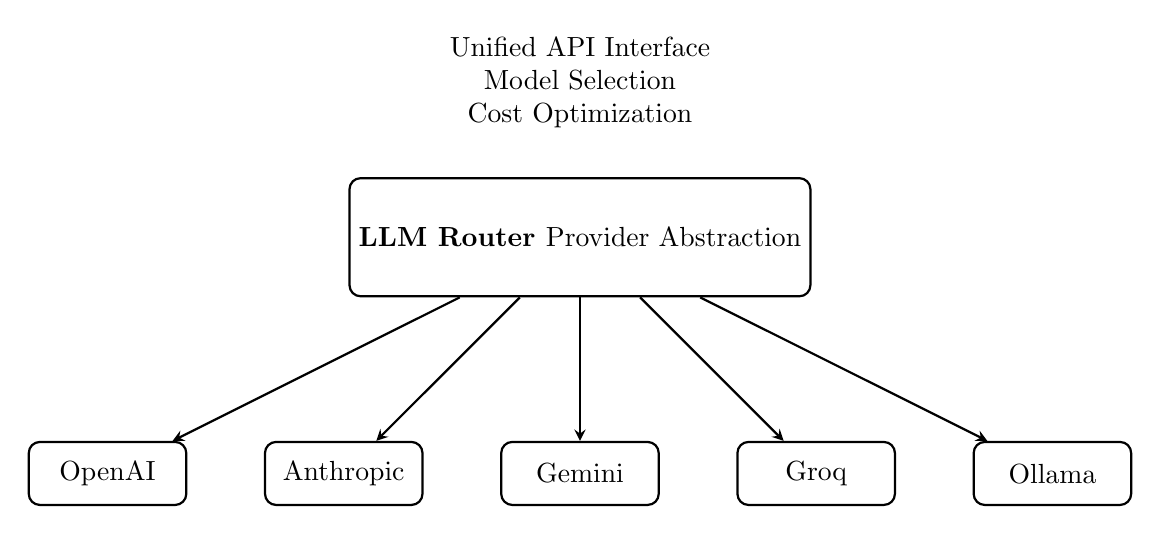
\begin{tikzpicture}[
    node distance=1.5cm,
    provider/.style={rectangle, rounded corners, draw, thick, minimum width=2cm, minimum height=0.8cm, fill=white},
    router/.style={rectangle, draw, thick,rounded corners, minimum width=3cm, minimum height=1.5cm, fill=white},
    arrow/.style={->, >=stealth, thick}
]
    \node[router] (router) at (6,0) {\textbf{LLM Router  } \newline Provider Abstraction};
    
    \node[provider] (openai) at (0,-3) {OpenAI};
    \node[provider] (anthropic) at (3,-3) {Anthropic};
    \node[provider] (gemini) at (6,-3) {Gemini};
    \node[provider] (groq) at (9,-3) {Groq};
    \node[provider] (ollama) at (12,-3) {Ollama};
    
    \draw[arrow] (router) -- (openai);
    \draw[arrow] (router) -- (anthropic);
    \draw[arrow] (router) -- (gemini);
    \draw[arrow] (router) -- (groq);
    \draw[arrow] (router) -- (ollama);
    
    \node[above=0.5cm of router, align=center] {Unified API Interface \\ Model Selection \\ Cost Optimization};
\end{tikzpicture}
\caption{LLM Provider Integration Architecture}
\end{figure}

\subsection*{\textbf{3.9 Data Flow Architecture}}

\begin{figure}[h]
\centering
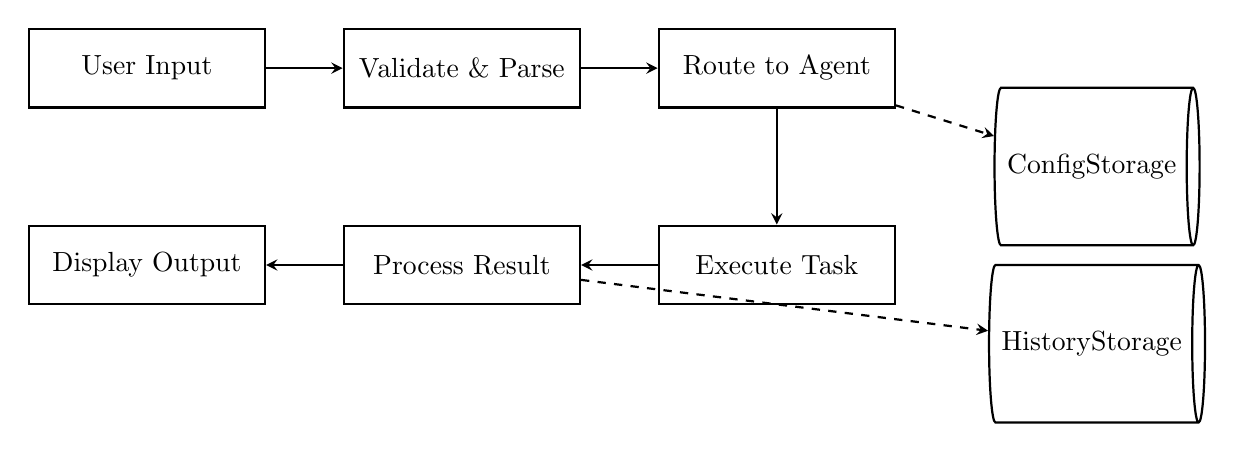
\begin{tikzpicture}[
    node distance=1.5cm,
    process/.style={rectangle, draw, thick, minimum width=3cm, minimum height=1cm, fill=white},
    storage/.style={cylinder, draw, thick, minimum width=2cm, minimum height=1.2cm, fill=white, shape aspect=0.3},
    arrow/.style={->, >=stealth, thick}
]
    \node[process] (input) at (0,0) {User Input};
    \node[process] (validate) at (4,0) {Validate \& Parse};
    \node[process] (route) at (8,0) {Route to Agent};
    \node[process] (execute) at (8,-2.5) {Execute Task};
    \node[process] (result) at (4,-2.5) {Process Result};
    \node[process] (output) at (0,-2.5) {Display Output};
    
    \node[storage] (config) at (12,-1.25) {Config \newline Storage};
    \node[storage] (history) at (12,-3.5) {History \newline Storage};
    
    \draw[arrow] (input) -- (validate);
    \draw[arrow] (validate) -- (route);
    \draw[arrow] (route) -- (execute);
    \draw[arrow] (execute) -- (result);
    \draw[arrow] (result) -- (output);
    
    \draw[arrow, dashed] (route) -- (config);
    \draw[arrow, dashed] (result) -- (history);
\end{tikzpicture}
\caption{Data Flow and Processing Architecture}
\end{figure}

\newpage

\subsection*{\textbf{3.10 Execution Pipeline Detail}}

The execution lifecycle combines deterministic orchestration with adaptive AI reasoning:

\begin{enumerate}
    \item \textbf{Task Initialization:}
    \begin{itemize}
        \item Background service worker validates API providers
        \item Hydrates agent model selections from user settings
        \item Applies firewall rules and general configuration
        \item Instantiates Executor with step limits and failure thresholds
    \end{itemize}
    
    \item \textbf{Context Construction:}
    \begin{itemize}
        \item Executor provisions AgentContext for shared state
        \item MessageManager handles conversation history
        \item EventManager tracks telemetry and status updates
        \item ActionBuilder provides DOM interaction utilities
    \end{itemize}
    
    \item \textbf{Thinker Planning Loop:}
    \begin{itemize}
        \item Runs at configurable intervals (default: every 3 steps)
        \item Produces strategic plans with reasoning and next steps
        \item Identifies potential challenges and edge cases
        \item Can terminate task early when \texttt{done=true}
        \item Plans persisted to history for debugging
    \end{itemize}
    
    \item \textbf{Navigator Action Loop:}
    \begin{itemize}
        \item Consumes shared memory and current browser state
        \item Samples DOM structure and interactive elements
        \item Predicts optimal multi-action sequences
        \item Executes actions with retry logic
        \item Records results and state snapshots
    \end{itemize}
    
    \item \textbf{Event System and Analytics:}
    \begin{itemize}
        \item Emits structured events: TASK\_START, STEP\_OK/FAIL
        \item Feeds real-time UI updates
        \item Powers telemetry dashboard
        \item Enables replay and debugging
    \end{itemize}
    
    \item \textbf{Cleanup and Replay:}
    \begin{itemize}
        \item Browser contexts properly disposed
        \item Action history serialized for replay
        \item Deterministic regression testing enabled
        \item Performance metrics collected
    \end{itemize}
\end{enumerate}

\subsection*{\textbf{3.11 Error Handling and Recovery}}

\begin{figure}[h]
\centering
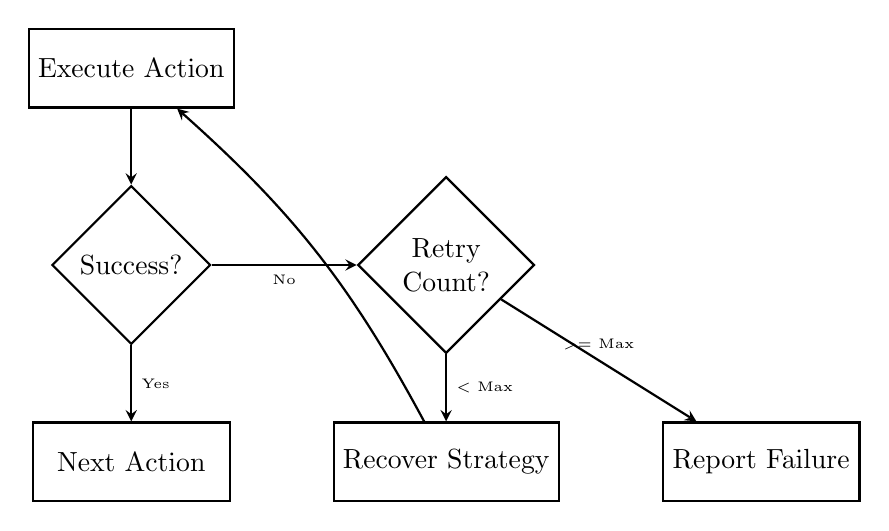
\begin{tikzpicture}[
    node distance=2cm,
    decision/.style={diamond, draw, thick, minimum width=2cm, minimum height=2cm, fill=white, align=center},
    process/.style={rectangle, draw, thick, minimum width=2.5cm, minimum height=1cm, fill=white},
    arrow/.style={->, >=stealth, thick}
]
    \node[process] (action) at (0,0) {Execute Action};
    \node[decision] (check) at (0,-2.5) {Success?};
    \node[decision] (retry) at (4,-2.5) {Retry \\ Count?};
    \node[process] (recover) at (4,-5) {Recover Strategy};
    \node[process] (fail) at (8,-5) {Report Failure};
    \node[process] (next) at (0,-5) {Next Action};
    
    \draw[arrow] (action) -- (check);
    \draw[arrow] (check) -- node[left,below, font=\tiny] {No} (retry);
    \draw[arrow] (check) -- node[right, font=\tiny] {Yes} (next);
    \draw[arrow] (retry) -- node[right, font=\tiny] {< Max} (recover);
    \draw[arrow] (retry) -- node[above, font=\tiny] {>= Max} (fail);
    \draw[arrow] (recover) to[bend right=10] (action);
\end{tikzpicture}
\caption{Error Handling and Recovery Flow}
\end{figure}

\newpage

% ==================== 4. EXPECTED CONTRIBUTION ====================
\section*{\textbf{4. EXPECTED CONTRIBUTION FROM THE STUDY}}
\addcontentsline{toc}{section}{4. EXPECTED CONTRIBUTION FROM THE STUDY}

This project contributes significantly to the field of AI and web automation:

\vspace{0.3cm}

\subsection*{\textbf{4.1 Technical Contributions}}

\begin{enumerate}
    \item \textbf{Open-Source Multi-Agent Framework:} Provides a reusable architecture for building collaborative AI agents in browser environments
    
    \item \textbf{Privacy-Preserving AI:} Demonstrates feasibility of running sophisticated AI workflows entirely client-side without server dependency
    
    \item \textbf{Provider-Agnostic LLM Integration:} Establishes patterns for flexible AI model integration that reduces vendor lock-in
    
    \item \textbf{Browser Extension Architecture:} Showcases modern Manifest V3 development practices with React and TypeScript
    
    \item \textbf{Cost Optimization Strategies:} Implements intelligent caching and model selection to minimize API expenses
\end{enumerate}

\subsection*{\textbf{4.2 Social and Economic Impact}}

\begin{enumerate}
    \item \textbf{Democratization of Technology:} Removes financial barriers to advanced web automation, making it accessible to students, researchers, and small businesses
    
    \item \textbf{Educational Resource:} Serves as learning material for AI integration, browser APIs, and modern web development
    
    \item \textbf{Community Building:} Fosters collaborative development through Discord, GitHub, and comprehensive documentation
    
    \item \textbf{Cost Savings:} Enables users to save thousands of dollars annually compared to commercial alternatives
    
    \item \textbf{Privacy Advocacy:} Promotes data sovereignty and local-first computing principles
\end{enumerate}

\subsection*{\textbf{4.3 Research Contributions}}

\begin{enumerate}
    \item \textbf{Multi-Agent Coordination:} Explores effective collaboration patterns between specialized AI agents
    
    \item \textbf{Browser Automation Intelligence:} Studies adaptive strategies for handling dynamic web content
    
    \item \textbf{Human-AI Interaction:} Investigates natural language interfaces for complex task automation
    
    \item \textbf{Performance Benchmarking:} Provides data on different LLM models' effectiveness for web automation tasks
\end{enumerate}

\subsection*{\textbf{4.4 Future Applications}}

The technologies and patterns developed in this project can be extended to:

\begin{itemize}
    \item Automated testing frameworks for web applications
    \item Research data collection and analysis tools
    \item Accessibility tools for users with disabilities
    \item Workflow automation for business processes
    \item Educational tools for teaching programming and AI
    \item Browser-based AI assistants for various domains
\end{itemize}

\newpage

% ==================== 5. ACTIVITIES ====================
\section*{\textbf{5. LIST OF ACTIVITIES CARRIED OUT TO COMPLETE THE PROJECT}}
\addcontentsline{toc}{section}{5. LIST OF ACTIVITIES CARRIED OUT TO COMPLETE THE PROJECT}

\subsection*{\textbf{5.1 Project Phases and Activities}}

\begin{enumerate}
    \item \textbf{Phase 1: Planning and Requirements Analysis} (8 days)
    \begin{itemize}
        \item Market research and competitive analysis
        \item User requirement gathering
        \item Technology stack evaluation
        \item Architecture design planning
        \item Risk assessment and mitigation strategies
    \end{itemize}
    
    \item \textbf{Phase 2: System Architecture Design} (12 days)
    \begin{itemize}
        \item Monorepo structure design
        \item Chrome extension manifest planning
        \item Multi-agent system architecture
        \item Database and storage schema design
        \item API integration design
        \item Security and privacy framework
    \end{itemize}
    
    \item \textbf{Phase 3: Core Development} (20 days)
    \begin{itemize}
        \item Background service worker implementation
        \item Content script development
        \item Message passing system
        \item Storage management layer
        \item Event handling system
        \item Error handling and logging
    \end{itemize}
    
    \item \textbf{Phase 4: AI Integration and Agent Development} (15 days)
    \begin{itemize}
        \item OpenAI API integration and testing
        \item Anthropic Claude integration
        \item Google Gemini integration
        \item Groq and Ollama support
        \item Custom provider interface
        \item Multi-agent orchestration logic
        \item Navigator agent implementation
        \item Thinker agent implementation
    \end{itemize}
    
    \item \textbf{Phase 5: User Interface Development} (18 days)
    \begin{itemize}
        \item React component architecture
        \item Side panel interface design
        \item Settings page implementation
        \item Conversation history UI
        \item Real-time status updates
        \item Responsive design and accessibility
        \item Dark mode support
        \item Loading states and animations
    \end{itemize}
    
    \item \textbf{Phase 6: Testing and Quality Assurance} (14 days)
    \begin{itemize}
        \item Unit test development
        \item Integration testing
        \item End-to-end automation testing
        \item Cross-browser compatibility testing
        \item Performance optimization
        \item Security vulnerability assessment
        \item User acceptance testing
    \end{itemize}
    
    \item \textbf{Phase 7: Documentation} (10 days)
    \begin{itemize}
        
        \item API reference documentation
        
        
        \item Installation and setup guides
        \item Troubleshooting documentation
        \item Video tutorials planning
    \end{itemize}
    
    \item \textbf{Phase 8: Deployment and Publishing} (8 days)
    \begin{itemize}
        \item Chrome Web Store submission
        \item Extension review process
        \item Marketing materials creation
        \item Website and landing page
    
    \item \textbf{Phase 9: Community Building} (6 days)
    \begin{itemize}
        \item Discord server setup and moderation
        \item GitHub Discussions activation
        \item Community guidelines
        \item User onboarding process
    \end{itemize}
    
    \item \textbf{Phase 10: Maintenance and Updates} (10 days)
    \begin{itemize}
        \item Bug fixes and patches
        \item Feature implementation based on feedback
        \item Performance optimization
        \item Security updates
        \item Version releases (v0.1.1 - v0.1.12)
        \item Documentation updates
    \end{itemize}
\end{enumerate}



\subsection*{\textbf{5.2 Project Timeline Visualization}}

\begin{figure}[h]
\centering
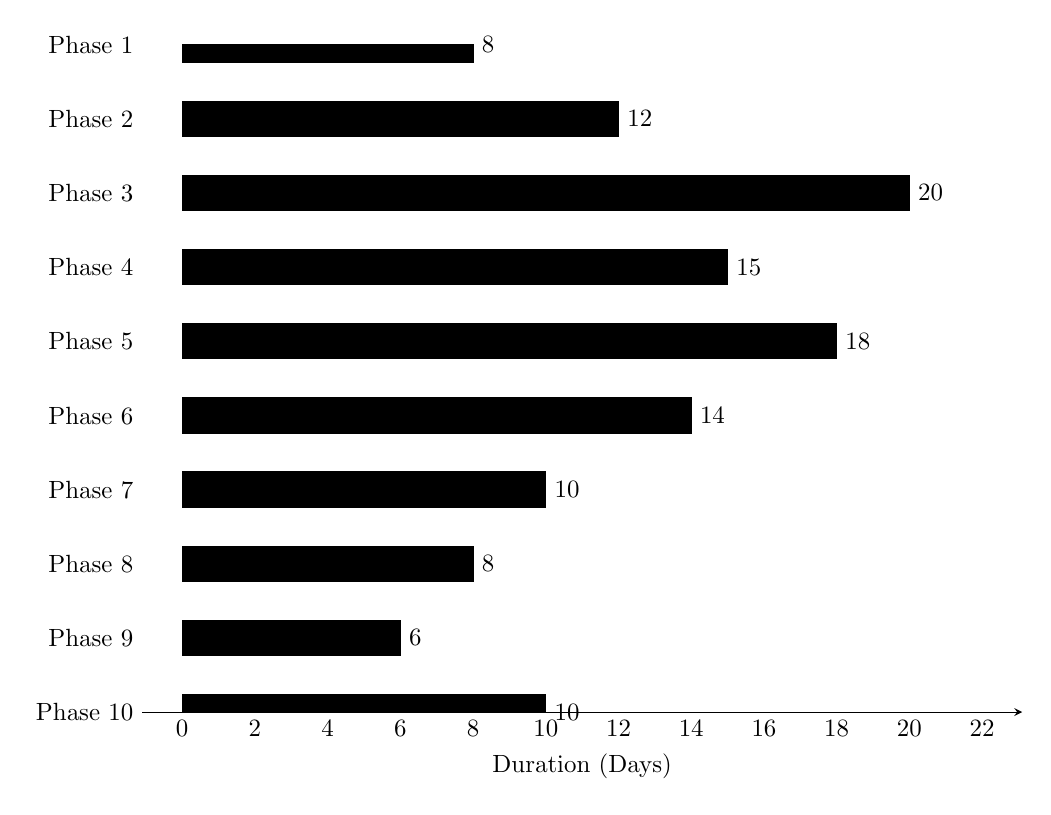
\begin{tikzpicture}[scale=0.9, transform shape]
    \begin{axis}[
        xbar,
        width=14cm,
        height=11cm,
        y axis line style = { opacity = 0 },
        axis x line = bottom,
        tickwidth = 0pt,
        enlarge y limits = 0,
        enlarge x limits = 0.05,
        symbolic y coords = {Phase 10,Phase 9,Phase 8,Phase 7,Phase 6,Phase 5,Phase 4,Phase 3,Phase 2,Phase 1},
        nodes near coords,
        nodes near coords align = horizontal,
        xlabel = {Duration (Days)},
        xmin=0,
        xmax=22,
        bar width=0.5cm,
    ]
        \addplot[fill=black] coordinates {
            (10,Phase 10)
            (6,Phase 9)
            (8,Phase 8)
            (10,Phase 7)
            (14,Phase 6)
            (18,Phase 5)
            (15,Phase 4)
            (20,Phase 3)
            (12,Phase 2)
            (8,Phase 1)
        };
    \end{axis}
\end{tikzpicture}
\caption{Project Timeline - Total Duration: 121 Days}
\end{figure}
\newpage

\subsection*{\textbf{5.3 Resource Allocation}}

\begin{table}[h]
\centering
\begin{tabular}{|l|c|c|c|}
\hline
\textbf{Phase} & \textbf{Duration} & \textbf{Effort (\%)} & \textbf{Priority} \\
\hline
Planning & 8 days & 6.6\% & High \\
\hline
Architecture & 12 days & 9.9\% & High \\
\hline
Core Development & 20 days & 16.5\% & Critical \\
\hline
AI Integration & 15 days & 12.4\% & Critical \\
\hline
UI Development & 18 days & 14.9\% & High \\
\hline
Testing & 14 days & 11.6\% & Critical \\
\hline
Documentation & 10 days & 8.3\% & Medium \\
\hline
Deployment & 8 days & 6.6\% & High \\
\hline
Community & 6 days & 5.0\% & Medium \\
\hline
Maintenance & 10 days & 8.3\% & Ongoing \\
\hline
\textbf{Total} & \textbf{121 days} & \textbf{100\%} & - \\
\hline
\end{tabular}
\caption{Resource Allocation Across Project Phases}
\end{table}

\subsection*{\textbf{5.4 Milestone Timeline}}

\begin{figure}[h]
\centering
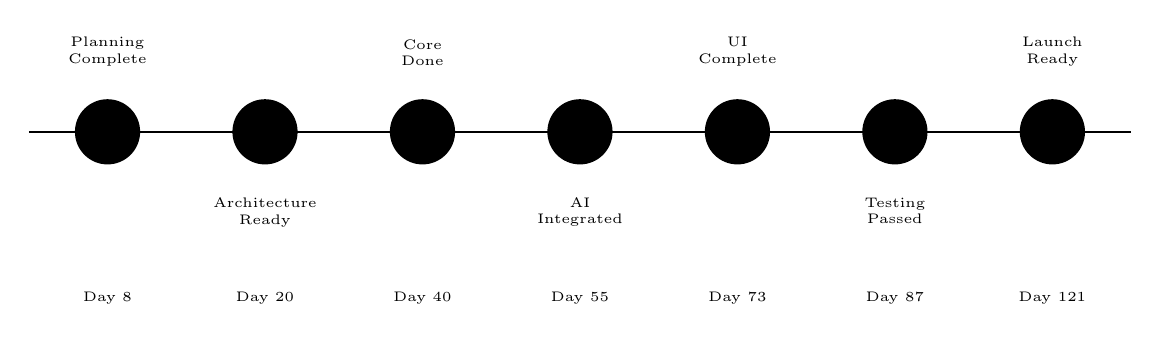
\begin{tikzpicture}[
    milestone/.style={circle, draw, thick, minimum size=0.8cm, fill=black},
    arrow/.style={->, >=stealth, thick}
]
    % Timeline
    \draw[thick] (0,0) -- (14,0);
    
    % Milestones
    \node[milestone] (m1) at (1,0) {};
    \node[above=0.3cm of m1, align=center, font=\tiny] {Planning\\Complete};
    
    \node[milestone] (m2) at (3,0) {};
    \node[below=0.3cm of m2, align=center, font=\tiny] {Architecture\\Ready};
    
    \node[milestone] (m3) at (5,0) {};
    \node[above=0.3cm of m3, align=center, font=\tiny] {Core\\Done};
    
    \node[milestone] (m4) at (7,0) {};
    \node[below=0.3cm of m4, align=center, font=\tiny] {AI\\Integrated};
    
    \node[milestone] (m5) at (9,0) {};
    \node[above=0.3cm of m5, align=center, font=\tiny] {UI\\Complete};
    
    \node[milestone] (m6) at (11,0) {};
    \node[below=0.3cm of m6, align=center, font=\tiny] {Testing\\Passed};
    
    \node[milestone] (m7) at (13,0) {};
    \node[above=0.3cm of m7, align=center, font=\tiny] {Launch\\Ready};
    
    % Time labels
    \node[below=1.5cm of m1] {\tiny Day 8};
    \node[below=1.5cm of m2] {\tiny Day 20};
    \node[below=1.5cm of m3] {\tiny Day 40};
    \node[below=1.5cm of m4] {\tiny Day 55};
    \node[below=1.5cm of m5] {\tiny Day 73};
    \node[below=1.5cm of m6] {\tiny Day 87};
    \node[below=1.5cm of m7] {\tiny Day 121};
\end{tikzpicture}
\caption{Project Milestone Timeline}
\end{figure}

\newpage

% ==================== 6. TOOLS AND EQUIPMENT ====================
\section*{\textbf{6. PLACES/LABS/EQUIPMENT AND TOOLS USED}}
\addcontentsline{toc}{section}{6. PLACES/LABS/EQUIPMENT AND TOOLS USED}

\subsection*{\textbf{6.1 Development Environment}}

\begin{itemize}
    \item \textbf{Operating Systems:}
    \begin{itemize}
        \item Windows 10/11 (Primary development)
        \item macOS Sonoma/Ventura (Cross-platform testing)
        \item Ubuntu 22.04 LTS (Linux compatibility)
    \end{itemize}
    
    \item \textbf{Code Editors and IDEs:}
    \begin{itemize}
        \item Visual Studio Code (v1.85+) - Primary IDE
        \item WebStorm 2024.1 - Advanced JavaScript/TypeScript development
        \item Chrome DevTools - Debugging and profiling
    \end{itemize}
    
    \item \textbf{Browsers for Testing:}
    \begin{itemize}
        \item Google Chrome (v120+)
        \item Microsoft Edge (v120+)
        \item Chrome Canary (Latest features testing)
    \end{itemize}
    
    \item \textbf{Version Control:}
    \begin{itemize}
        \item Git (v2.42+)
        \item GitHub (Repository hosting and collaboration)
        \item GitHub Desktop (GUI for version control)
    \end{itemize}
\end{itemize}

\subsection*{\textbf{6.2 Development Tools and Libraries}}

\begin{table}[h]
\centering
\small
\begin{tabular}{|l|l|p{8cm}|}
\hline
\textbf{Tool/Library} & \textbf{Version} & \textbf{Purpose} \\
\hline
Node.js & 22.12.0+ & JavaScript runtime environment \\
\hline
pnpm & 9.15.1 & Fast, disk space efficient package manager \\
\hline
Turbo & 2.5.3 & Monorepo build system and task runner \\
\hline
Vite & 6.3.6 & Next-generation frontend build tool \\
\hline
TypeScript & 5.5.4 & Type-safe JavaScript superset \\
\hline
React & 18.3.1 & UI component library and framework \\
\hline
Tailwind CSS & 3.4.17 & Utility-first CSS framework \\
\hline
ESLint & 8.57.0 & Code quality and linting tool \\
\hline
Prettier & 3.3.3 & Opinionated code formatter \\
\hline
Husky & 9.1.4 & Git hooks automation tool \\
\hline
Zustand & 4.5.2 & State management library \\
\hline
React Router & 6.22.0 & Client-side routing \\

\hline
Zod & 3.22.4 & TypeScript-first schema validation \\
\hline
\end{tabular}
\caption{Development Tools and Libraries}
\end{table}
\newpage

\subsection*{\textbf{6.3 External APIs and Services}}

\begin{table}[h]
\centering
\small
\begin{tabular}{|l|p{8cm}|}
\hline
\textbf{Service} & \textbf{Purpose and Models} \\
\hline
OpenAI & GPT-4, GPT-4o, GPT-4o-mini, GPT-3.5-turbo models for task execution \\
\hline
Anthropic & Claude 3.5 Sonnet, Claude 3 Haiku models for reasoning tasks \\
\hline
Google Gemini & Gemini 2.5 Flash for fast inference and cost optimization \\
\hline
Groq & High-speed inference for real-time automation \\
\hline
Ollama & Local model deployment for privacy-focused users \\
\hline
Chrome Web Store & Extension distribution and version management \\
\hline
GitHub & Repository hosting, issue tracking, CI/CD \\
\hline
Discord & Community engagement and support platform \\
\hline
\end{tabular}
\caption{External APIs and Services}
\end{table}



\subsection*{\textbf{6.4 Development Standards and Best Practices}}

\begin{itemize}
    \item \textbf{Code Style Guidelines:}
    \begin{itemize}
        \item Airbnb ESLint configuration for JavaScript/TypeScript
        \item Prettier with 2-space indentation and single quotes
        \item Consistent file naming conventions (kebab-case)
        \item Component-based architecture for React
    \end{itemize}
    
    \item \textbf{Type Safety:}
    \begin{itemize}
        \item Strict TypeScript compiler options
        \item Comprehensive type definitions for all modules
        \item Zod schemas for runtime validation
        \item No implicit any types allowed
    \end{itemize}
    
    \item \textbf{Testing Standards:}
    \begin{itemize}
        \item End-to-end tests for critical user flows
        \item Manual testing across multiple websites
        \item Cross-browser compatibility testing
        \item Performance benchmarking
    \end{itemize}
    
    \item \textbf{Documentation Standards:}
    \begin{itemize}
        \item Markdown format for all documentation
        \item JSDoc comments for public APIs
        \item Code examples in documentation
        \item Architecture decision records (ADRs)
    \end{itemize}
    
    \item \textbf{Version Control Practices:}
    \begin{itemize}
        \item Meaningful commit messages following conventional commits
        \item Feature branches for new development
        \item Pull request reviews before merging
        \item Semantic versioning for releases
    \end{itemize}
\end{itemize}



\subsection*{\textbf{6.5 Hardware Requirements for Development}}

\begin{table}[h]
\centering
\begin{tabular}{|l|l|l|}
\hline
\textbf{Component} & \textbf{Minimum} & \textbf{Recommended} \\
\hline
Processor & Intel i5 / AMD Ryzen 5 & Intel i7 / AMD Ryzen 7 \\
\hline
RAM & 8 GB & 16 GB or more \\
\hline
Storage & 10 GB free space & 20 GB SSD \\
\hline
Internet & Stable connection & High-speed broadband \\
\hline
Display & 1366x768 & 1920x1080 or higher \\
\hline
\end{tabular}
\caption{Hardware Requirements for Development}
\end{table}

\newpage

% ==================== 7. REFERENCES ====================
\section*{\textbf{7. REFERENCES}}
\addcontentsline{toc}{section}{7. REFERENCES}

\setlength{\parindent}{0pt}
\setlength{\leftskip}{0.5in}
\setlength{\parskip}{0.25cm}

\noindent Anthropic. (2024). \textit{Claude API Documentation.} Retrieved from https://docs.anthropic.com

\noindent Browser Use. (2024). \textit{Browser Use - Open Source Browser Automation.} Retrieved from https://github.com/browser-use/browser-use

\noindent Chrome Extension Boilerplate. (2024). \textit{Chrome Extension Boilerplate React Vite.} Retrieved from https://github.com/Jonghakseo/chrome-extension-boilerplate-react-vite

\noindent Cosmos Team. (2024). \textit{Cosmos - AI Web Automation Tool.} Retrieved from https://github.com/cosmos/cosmos

\noindent Discord. (2024). \textit{Discord Developer Documentation.} Retrieved from https://discord.com/developers/docs

\noindent Emergence AI. (2024). \textit{Agent-E - Browser Automation.} Retrieved from https://github.com/EmergenceAI/Agent-E

\noindent Goodfellow, I., Bengio, Y., \& Courville, A. (2016). \textit{Deep Learning.} MIT Press.

\noindent Google. (2024). \textit{Chrome Extension Manifest V3 Documentation.} Retrieved from https://developer.chrome.com/docs/extensions/mv3/

\noindent Google. (2024). \textit{Google Gemini API Documentation.} Retrieved from https://ai.google.dev/docs

\noindent Groq. (2024). \textit{Groq API Documentation.} Retrieved from https://console.groq.com/docs

\noindent LangChain. (2024). \textit{LangChain JavaScript Documentation.} Retrieved from https://js.langchain.com

\noindent Meta. (2024). \textit{React 18 Documentation.} Retrieved from https://react.dev

\noindent Microsoft. (2024). \textit{TypeScript Handbook.} Retrieved from https://www.typescriptlang.org/docs

\noindent Mozilla. (2024). \textit{Web Extensions API.} Retrieved from https://developer.mozilla.org/en-US/docs/Mozilla/Add-ons/WebExtensions

\noindent OpenAI. (2024). \textit{OpenAI API Documentation.} Retrieved from https://platform.openai.com/docs

\noindent pnpm. (2024). \textit{pnpm Documentation.} Retrieved from https://pnpm.io

\noindent Puppeteer. (2024). \textit{Puppeteer - Headless Browser Automation.} Retrieved from https://pptr.dev

\noindent Russell, S., \& Norvig, P. (2020). \textit{Artificial Intelligence: A Modern Approach} (4th ed.). Pearson.

\noindent Tailwind Labs. (2024). \textit{Tailwind CSS Documentation.} Retrieved from https://tailwindcss.com/docs

\noindent The Turbo Team. (2024). \textit{Turbo Monorepo Tool Documentation.} Retrieved from https://turbo.build

\noindent Vaswani, A., Shazeer, N., Parmar, N., Uszkoreit, J., Jones, L., Gomez, A. N., Kaiser, L., \& Polosukhin, I. (2017). Attention Is All You Need. \textit{Advances in Neural Information Processing Systems, 30.}

\noindent Vercel. (2024). \textit{Husky - Git Hooks.} Retrieved from https://typicode.github.io/husky

\noindent Vite Team. (2024). \textit{Vite Documentation.} Retrieved from https://vitejs.dev

\noindent W3C. (2024). \textit{Web Accessibility Initiative (WAI).} Retrieved from https://www.w3.org/WAI/

\noindent Wooldridge, M. (2009). \textit{An Introduction to MultiAgent Systems} (2nd ed.). Wiley.

\end{document}